% !TeX document-id = {d8b4925c-2057-42a4-b894-2f1a3f1b6345}
%!TeX TXS-program:compile = txs:///xelatex/[--shell-escape]
\documentclass[aspectratio=169, mathserif]{beamer}	% TPU recommends 16:9 ratio, 4:3 may require some work with inner theme .sty file

% Style options:
% light --- light theme (default)
% dark --- dark theme
% enlogo --- english TPU logo {default}
% rulogo --- russian TPU logo

\usetheme[light, rulogo]{tpu}		% dark theme used as an example of optional argument

\usepackage[english, russian]{babel}		%uncomment this to work in russian
\usepackage[utf8]{inputenc}
\usepackage[T2A]{fontenc}

\usepackage{fontspec}

\setromanfont{Brygada1918}[
Path=./fonts/BrygadaFontFiles/,
Extension = .ttf,
UprightFont=*-Regular,
BoldFont=*-Bold,
ItalicFont=*-Italic,
BoldItalicFont=*-BoldItalic
]

\setsansfont{ALSSirius}[
Path=./fonts/ALSSiriusFiles/,
Extension = .otf,
UprightFont=*-Regular,
BoldFont=*-Bold,
%ItalicFont=*-Italic,
%BoldItalicFont=*-BoldItalic
]

\setmonofont{Consolas}[
Path=./fonts/ConsolasFontFiles/,
%Scale=0.85,
Extension = .ttf,
UprightFont=*-Regular,
BoldFont=*-Bold,
ItalicFont=*-Italic,
BoldItalicFont=*-BoldItalic
]

\usepackage[cache=false]{minted}
\usepackage{xcolor} % to access the named colour LightGray
\definecolor{LightGray}{gray}{0.9}
\definecolor{onedarkBckGr}{RGB}{40, 44, 52}

\usemintedstyle[python]{default}
\setminted[python]{
	fontsize=\scriptsize,
	escapeinside=||,
	mathescape=true,
	numbersep=5pt,
	gobble=2,
	linenos=true,
	frame=leftline,
	framesep=1mm,
	python3=true,
}

\usemintedstyle[pycon]{default}
\setminted[pycon]{
	fontsize=\scriptsize,
	escapeinside=||,
	mathescape=true,
	numbersep=5pt,
	gobble=2,
	linenos=false,
	frame=single,
	framesep=1mm,
	python3=true,
%	bgcolor=backcolour,
	linenos=true,
}

%\defaultfontfeatures{Ligatures={TeX},Renderer=Basic}  %% свойства шрифтов по умолчанию
%\setmainfont[Ligatures={TeX,Historic}]{Times New Roman} %% задаёт основной шрифт документа
%\setsansfont{Comic Sans MS}                    %% задаёт шрифт без засечек
%\setmonofont{Courier New}
%\usepackage[default]{droidserif}
%\usepackage[defaultsans]{droidsans}

\usepackage{booktabs}	% good looking tables
\usepackage{multicol}	% text in multiple columns, useful for side-by-side text and pictures
\usepackage{hyperref}
%\usepackage{minted}
\usepackage{xcolor}
\definecolor{maroon}{cmyk}{0, 0.87, 0.68, 0.32}
\definecolor{halfgray}{gray}{0.55}
\definecolor{ipython_frame}{RGB}{207, 207, 207}
\definecolor{ipython_bg}{RGB}{247, 247, 247}
\definecolor{ipython_red}{RGB}{186, 33, 33}
\definecolor{ipython_green}{RGB}{0, 128, 0}
\definecolor{ipython_cyan}{RGB}{64, 128, 128}
\definecolor{ipython_purple}{RGB}{170, 34, 255}
\definecolor{linkcolor}{HTML}{0000FF} % цвет гиперссылок
\definecolor{urlcolor}{HTML}{800080} % цвет ссылок
\definecolor{backcolour}{rgb}{0.95,0.95,0.92}

\usepackage{amsxtra}
\usepackage{longtable}
\usepackage{wrapfig}
\usepackage{ragged2e}
\usepackage[nooneline]{caption}
\DeclareCaptionTextFormat{center}{\centering{#1}}
\DeclareCaptionLabelFormat{figure}{Рисунок~#2}
\captionsetup[table]{justification=raggedleft,
	labelformat=empty,
	labelsep=endash,
	textformat=center,
	position=top,
	skip=5pt
}
\captionsetup[figure]{justification=centering,
	labelsep=endash,
	labelformat=figure,
	font={tiny}
}


\hyphenpenalty=10000	% i don’t think hyphenation in presentations is a good idea, feel free to change however you like

%\includeonlyframes{c}

\title{\LARGE{Системный анализ процессов химической технологии}}
\subtitle{\textcolor{tpugreen}{\textbf{Лекция 8}} \\ \textbf{Моделирование химических реакций}}
\author[]{\textbf{Вячеслав Алексеевич Чузлов}}
\institute{к.т.н., доцент ОХИ ИШПР}
\date{\today}

\begin{document}

% notice usage of \titleframe and several other unconventional functions
% the reason being is custom backgrounds on these slides

\titleframe		% title

\tocframe{}		% this custom frame accepts options for ToC

%\addcontentsline{toc}{section}{\textbf{I Численные методы решения систем \\ линейных уравнений}}


\begin{frame}[fragile, ]{Численные методы решения систем \\ дифференциальных уравнений}
\scriptsize
Задачи, в которых необходимо решить систему из нескольких дифференциальных уравнений с несколькими искомыми функциями, очень распространены в предметной области химической технологии.
\vfill
Будем рассматривать системы, в которых число неизвестных функций совпадает с числом уравнений, разрешенных относительно производных.
\vfill
К примеру, система из двух уравнений с двумя неизвестными функциями $y$ и $z$ от одного и того же аргумента $x$ имеет вид:
\vfill
\begin{equation}\label{system-ODE}
	\left\{
	\begin{aligned}
		y' &= f_1\left(x, y, z\right)\\
		z' &= f_2\left(x, y, z\right)
	\end{aligned}
	\right.
\end{equation}
\vfill
\noindent при этом штрих означает производную по $x$.
\vfill
\end{frame}


\begin{frame}[fragile, ]{Численные методы решения систем \\ дифференциальных уравнений}
\scriptsize
Общий вид системы из $n$ уравнений с $n$ неизвестными функциями $x_1, x_2, \ldots, x_n$ от переменной $t$ имеет вид:
\vfill
\begin{equation}\label{system-ODE2}
	\left\{
	\begin{aligned}
		\dfrac{dx_1}{dt} &= f_1\left(t, x_1, x_2, \ldots, x_n\right) \\
		\dfrac{dx_2}{dt} &= f_2\left(t, x_1, x_2, \ldots, x_n\right) \\
		\ldots & \\
		\dfrac{dx_n}{dt} &= f_n\left(t, x_1, x_2, \ldots, x_n\right)
	\end{aligned}
	\right.
\end{equation}
\vfill
Ранее мы рассмотрели численные методы решения обыкновенных дифференциальных уравнений вида $y'=f(x,y)$ (методы Эйлера и Рунге-Кутты). Данные методы применяются и в случае решения систем обыкновенных дифференциальных уравнений.
\vfill
\end{frame}


\section{Метод Эйлера}
\sectionframe

\begin{frame}[fragile, ]{Метод Эйлера}
\scriptsize
Пусть дана следующая система обыкновенных дифференциальных уравнений:
\vfill
\begin{equation}
	\left\{
	\begin{aligned}
		\dfrac{dy_1}{dx} &= f_1 \left(x, y_1, y_2\right) \\
		\dfrac{dy_2}{dx} &= f_2\left(x, y_1, y_2\right)
	\end{aligned}
	\right.
\end{equation}
\vfill
\noindent с начальными условиями:
\vfill
\begin{equation}
	\begin{aligned}
		y_1 \big |_{x=x_0} &= y_{01} \\
		y_2 \big |_{x=x_0} &= y_{02}
	\end{aligned}
\end{equation}
\vfill
При использовании метода Эйлера, расчетные формулы примут следующий вид:
\vfill
\begin{equation}\label{Eiler_system}
	\left\{
	\begin{aligned}
		y_{(i), 1} &= y_{i-1,1} + h \cdot f_1 \left(x_{i-1}, y_{(i-1),1}, y_{(i-1),2}\right) \\
		y_{(i), 2} &= y_{i-1,2} + h \cdot f_2 \left(x_{i-1}, y_{(i-1),1}, y_{(i-1),2}\right) \\
		x_{i} &= x_{i-1} + h
	\end{aligned}
	\right.
\end{equation}
\vfill
\noindent где $h$~-- шаг интегрирования; $f_1\left(x_i, y_{i, 1}, y_{i, 2}\right)$ и $f_2\left(x_i, y_{i, 1}, y_{i, 2}\right)$~-- правые части дифференциальных уравнений.
\vfill
\end{frame}


\subsection{Пример~1}
\begin{frame}[fragile, ]{Пример~1}\label{slide:example1}
\scriptsize
Пусть требуется решить систему дифференциальных уравнений первого порядка:
\vfill
\begin{equation*}
	\left\{
	\begin{aligned}
		\dfrac{dy_1}{dx} &= y_2 \\
		\dfrac{dy_2}{dx} &= e^{-x\cdot y_1}
	\end{aligned}
	\right.
\end{equation*}
\vfill
\noindent методом Эйлера на отрезке $[0, 1]$ с шагом $h=0.1$.
\vfill
Начальные условия: $x_0 = 0$; $y_1(0)=0$; $y_2(0)=0$.
\vfill
Воспользуемся формулой~\eqref{Eiler_system} и запишем выражения для $y_{i,1}$ и $y_{i,2}$:
\vfill
\begin{equation*}
	\left\{
	\begin{aligned}
		y_{i,1} &= y_{(i-1),1} + 0.1 \cdot y_{(i-1),2} \\
		y_{i,2} &= y_{(i-1),2} + 0.1 \cdot e^{-x_{i-1}\cdot y_{(i-1),1}} \\
		x_i &= x_{i-1} + h
	\end{aligned}
	\right.
\end{equation*}
\vfill
\end{frame}

\begin{frame}[fragile, ]{Пример~1}
\scriptsize
Результаты вычислений сведем в таблице.
\vfill
\renewcommand{\arraystretch}{1.5}
\begin{longtable}{|r|r|r|r|}
%	\caption{}
%	\label{tab:eiler_system} \\

	\hline \multicolumn{1}{|r|}{$i$} & \multicolumn{1}{r|}{$x_i$} & \multicolumn{1}{r|}{$y_{i,1} = y_{(i-1),1} + 0.1 \cdot y_{(i-1),2}$} & \multicolumn{1}{r|}{$y_{i,2} = y_{(i-1),2} + 0.1 \cdot e^{-x_{i-1}\cdot y_{(i-1),1}}$}  \\
	\hline
	\endfirsthead

	\multicolumn{4}{r}{Продолжение таблицы \thetable{}} \\
	\hline
	\multicolumn{1}{|r|}{$i$} & \multicolumn{1}{r|}{$x_i$} & \multicolumn{1}{r|}{$y_{i,1} = y_{(i-1),1} + 0.1 \cdot y_{(i-1),2}$} & \multicolumn{1}{r|}{$y_{i,2} = y_{(i-1),2} + 0.1 \cdot e^{-x_{i-1}\cdot y_{(i-1),1}}$}  \\
	\hline
	\endhead

	$0$  &$0.0$ & $0.0000$ & $0.0000$  \\
	\hline

	$1$  &$0.1$ & $0.0000$ & $0.1000$  \\
	\hline

	$2$  &$0.2$ & $0.0100$ & $0.2000$  \\
	\hline

	$3$  &$0.3$ & $0.0300$ & $0.2998$ \\
	\hline

	$4$  &$0.4$ & $0.0600$ & $0.3989$  \\
	\hline

	$5$  &$0.5$ & $0.0999$ & $0.4965$  \\
	\hline

	$6$  &$0.6$ & $0.1495$ & $0.5917$  \\
	\hline

	$7$  &$0.7$ & $0.2087$ & $0.6831$  \\
	\hline

	$8$  &$0.8$ & $0.2770$ & $0.7695$  \\
	\hline

	$9$  &$0.9$ & $0.3539$ & $0.8496$  \\
	\hline

	$10$  &$1.0$ & $0.4389$ & $0.9223$  \\
	\hline
\end{longtable}
\vfill
\end{frame}

\subsubsection{Программная реализация}
\begin{frame}[fragile, ]{Программная реализация}
\scriptsize
\begin{minted}{python}
import numpy as np


def eiler(func, x0, xf, y0, h):
    count = int((xf - x0) / h) + 1
    y = [y0[:]]  # создание массива y с начальными условиями
    x = x0

    for i in range(1, count):
        right_parts = func(x, y[i-1])
        y.append([])  # добавление пустой строки

        for j in range(len(y0)):
            y[i].append(y[i-1][j] + h * right_parts[j])

        x += h

    return y
|\space|
|\space|
\end{minted}
\vfill
\end{frame}


\begin{frame}[fragile]{Программная реализация}
\scriptsize
\begin{minted}[firstnumber=last]{python}
def equations(x, y):  # Функция, содержащая правые части дифференциальных уравнений
    return [y[1], np.exp(-x * y[0])]


if __name__ == '__main__':
    print(eiler(equations, 0, 1, [0, 0], 0.1))
|\space|
\end{minted}
\vfill
\begin{minted}[frame=none, linenos=false]{pycon}
[[0, 0],
 [0.0, 0.1],
 [0.010000000000000002, 0.2],
 [0.030000000000000006, 0.29980019986673334],
 [0.05998001998667334, 0.39890423774402173],
 [0.09987044376107551, 0.4965335889709902],
 [0.14952380265817453, 0.5916626935059732],
 [0.20869007200877185, 0.6830819284599525],
 [0.2769982648547671, 0.7694905222116074],
 [0.35394731707592786, 0.8496142128887387],
 [0.4389087383648017, 0.9223342965713657]]
\end{minted}
\vfill
\end{frame}

\subsection{Пример~2}
\begin{frame}[fragile]{Пример~2}
\scriptsize
\alert{\textbf{Закон действующих масс}}
\vfill
Скорость химической реакции прямо пропорциональна произведению концентраций реагирующих веществ, возведенных в степени, равные их стехиометрическим коэффициентам.
\vfill
\begin{multicols}{2}
Схема химической реакции:
\vfill
$$
	n_1A_1 + n_2A_2 + n_3A_3 \overset{k}{\longrightarrow} B
$$
\vfill
Скорость данной реакции:
\vfill
$$
r = k \cdot \left[A_1\right]^{n_1} \cdot \left[A_2\right]^{n_2} \cdot \left[A_3\right]^{n_3}
$$
\vfill
\columnbreak
Изменение концентрации каждого компонента во времени:
\vfill
\begin{equation*}
	\left\{
	\begin{aligned}
		\dfrac{\partial C_{A_1}}{\partial t} &= -n_1 \cdot r \\
		\dfrac{\partial C_{A_2}}{\partial t} &= -n_2 \cdot r \\
		\dfrac{\partial C_{A_3}}{\partial t} &= -n_3 \cdot r \\
		\dfrac{\partial C_B}{\partial t} &= r
	\end{aligned}
	\right.
\end{equation*}
\end{multicols}
\vfill
где $k$~-- константа скорости химической реакции; $C_{A_1}$, $C_{A_2}$, $C_{A_3}$, $C_B$~-- концентрации веществ (моль/л), участвующих в химической реакции, $n_1$, $n_2$, $n_3$~-- стехиометрические коэффициенты в уравнении реакции.
\vfill
\end{frame}


\begin{frame}[fragile]{Пример~2}\label{slide:example2}
\scriptsize
Пусть дана схема химических реакций:
\vfill
$$
A \overset{k_1}{\underset{k_2}{\rightleftarrows}} B
$$
\vfill
Скорость прямой реакции: $r_1 = k_1 \cdot C_A$; скорость обратной реакции:
$r_2 = k_2 \cdot C_B$. Константы скоростей реакций: $k_1 = 0.85$; $k_2 = 0.1$, $C_A$ и $C_B$~-- концентрации компонентов $A$ и $B$.
Изменение концентрации реагирующих веществ во времени описывается следующей системой дифференциальных уравнений:
\vfill
\begin{equation*}
	\left\{
	\begin{aligned}
		\dfrac{\partial C_A}{\partial t} &= -r_1 + r_2 \\
		\dfrac{\partial C_B}{\partial t} &= r_1 - r_2
	\end{aligned}
	\right.
\end{equation*}
\vfill
Необходимо определить изменение концентрации каждого компонента по времени методом Эйлера на отрезке $[0, 1]$ с  шагом $h=0.1$. Начальные условия: $C_A(0) = 1$~(моль/л); $C_B(0) = 0$~(моль/л).
\vfill
Воспользуемся формулой~\eqref{Eiler_system} и запишем выражения для $C_{A,i}$ и $C_{B,i}$:
\vfill
\begin{equation*}
	\left\{
	\begin{aligned}
		C_{A, i} &= C_{A, (i-1)} + 0.1 \cdot \left(-k_1\cdot C_{A, (i-1)} + k_2 \cdot C_{B, (i-1)}\right) \\
		C_{B, i} &= C_{B, (i-1)} + 0.1 \cdot \left(k_1\cdot C_{A, (i-1)} - k_2 \cdot C_{B, (i-1)}\right) \\
		t_i &= t_{i-1} + h
	\end{aligned}
	\right.
\end{equation*}
\vfill
\end{frame}


\begin{frame}[fragile]{Пример 2}
\scriptsize
\begin{equation*}
	\left\{
	\begin{aligned}
		C_{A, i} &= C_{A, (i-1)} + 0.1 \cdot \left(-k_1\cdot C_{A, (i-1)} + k_2 \cdot C_{B, (i-1)}\right) \\
		C_{B, i} &= C_{B, (i-1)} + 0.1 \cdot \left(k_1\cdot C_{A, (i-1)} - k_2 \cdot C_{B, (i-1)}\right) \\
		t_i &= t_{i-1} + h
	\end{aligned}
	\right.
\end{equation*}
Результаты вычислений сведем в таблице.
\vfill
\begin{longtable}{|r|r|r|r|}
%	\caption{}
%	\label{tab:eiler_system2} \\

	\hline \multicolumn{1}{|r|}{$i$} & \multicolumn{1}{r|}{$t_i$} & \multicolumn{1}{r|}{$C_{A,i}$} & \multicolumn{1}{r|}{$C_{B,i}$}  \\
	\hline
	\endfirsthead

	\multicolumn{4}{r}{Продолжение таблицы \thetable{}} \\
	\hline
	\multicolumn{1}{|r|}{$i$} & \multicolumn{1}{r|}{$t_i$} & \multicolumn{1}{r|}{$C_{A,i}$} & \multicolumn{1}{r|}{$C_{B,i}$}  \\
	\hline
	\endhead

	$0$  &$0.0$ & $1.0000$ & $0.0000$  \\
	\hline

	$1$  &$0.1$ & $0.9150$ & $0.0850$  \\
	\hline

	$2$  &$0.2$ & $0.8381$ & $0.1619$  \\
	\hline

	$3$  &$0.3$ & $0.7685$ & $0.2315$ \\
	\hline

	$4$  &$0.4$ & $0.7055$ & $0.2945$  \\
	\hline

	$5$  &$0.5$ & $0.6484$ & $0.3516$  \\
	\hline

	$6$  &$0.6$ & $0.5968$ & $0.4032$  \\
	\hline

	$7$  &$0.7$ & $0.5501$ & $0.4499$  \\
	\hline

	$8$  &$0.8$ & $0.5079$ & $0.4921$  \\
	\hline

	$9$  &$0.9$ & $0.4696$ & $0.5304$  \\
	\hline

	$10$  &$1.0$ & $0.4350$ & $0.5650$  \\
	\hline
\end{longtable}
\vfill
\end{frame}


\subsubsection{Программная реализация}
\begin{frame}[fragile]{Программная реализация}
\scriptsize
\begin{minted}{python}
def equations(t, c, k):  # Функция, содержащая правые части дифф. уравнений
    right_parts = [
        -k[0] * c[0] + k[1] * c[1],
        k[0] * c[0] - k[1] * c[1],
    ]
    return right_parts


def eiler(func, x0, xf, y0, h, args=()):
    count = int((xf - x0) / h) + 1
    y, x = [y0[:]], x0
    for i in range(1, count):
        right_parts = func(x, y[i-1], *args)
        y.append([])
        for j in range(len(y0)):
            y[i].append(y[i-1][j] + h * right_parts[j])
        x += h
    return y
|\space|
|\space|
\end{minted}
\vfill
\end{frame}


\begin{frame}[fragile, ]{Программная реализация}
\scriptsize
\begin{minted}[firstnumber=last]{python}
k = [0.85, 0.1]
print(eiler(equations, 0, 1, [1, 0], 0.1, args=(k, )))
|\space|
\end{minted}
\vfill
\begin{minted}[frame=none, linenos=false]{pycon}
[[1, 0],
 [0.915, 0.085],
 [0.838075, 0.16192500000000004],
 [0.7684578750000001, 0.23154212500000004],
 [0.7054543768750001, 0.29454562312500004],
 [0.6484362110718751, 0.35156378892812506],
 [0.596834771020047, 0.4031652289799532],
 [0.5501354677731425, 0.4498645322268577],
 [0.5078725983346939, 0.4921274016653062],
 [0.469624701492898, 0.5303752985071022],
 [0.4350103548510727, 0.5649896451489275]]
\end{minted}
\vfill
\end{frame}


\section{Метод Рунге-Кутты}
\sectionframe


\begin{frame}[fragile, ]{Метод Рунге-Кутты}
\scriptsize
Пусть дана следующая система обыкновенных дифференциальных уравнений:
\vfill
\begin{equation}
	\left\{
	\begin{aligned}
		\dfrac{dy_1}{dx} &= f_1 \left(x, y_1, y_2\right) \\
		\dfrac{dy_2}{dx} &= f_2\left(x, y_1, y_2\right)
	\end{aligned}
	\right.
\end{equation}
\vfill
\noindent с начальными условиями:
\vfill
\begin{equation}
	\begin{aligned}
		y_1 \big |_{x=x_0} &= y_{01} \\
		y_2 \big |_{x=x_0} &= y_{02}
	\end{aligned}
\end{equation}
\vfill
\end{frame}


\begin{frame}[fragile, ]{Метод Рунге-Кутты}
\scriptsize
При использовании метода Рунге-Кутты, расчетные формулы примут следующий вид:
\vfill
\begin{equation}\label{RK_system}
	\left\{
	\begin{aligned}
		y_{i, 1} &= y_{(i-1),1} + h / 6 \cdot \left(k_{1,1} + 2 \cdot k_{2,1} + 2 \cdot k_{3,1} + k_{4,1}\right) \\
		y_{i, 2} &= y_{(i-1),2} + h / 6 \cdot \left(k_{1,2} + 2 \cdot k_{2,2} + 2 \cdot k_{3,2} + k_{4,2}\right) \\
		x_{i} &= x_{i-1} + h
	\end{aligned}
	\right.
\end{equation}
\vfill
\noindent где
\vfill
\begin{equation}\label{RK-params-system}
	\begin{tiny}
		\begin{aligned}
			k_{1,1} &= f_1\left(x, y_{(i-1),1}, y_{(i-1),2}\right); &\space
			k_{1,2} &= f_2\left(x, y_{(i-1),1}, y_{(i-1),2}\right); \\
			k_{2,1} &= f_1 \left(x + \dfrac{h}{2}, y_{(i-1),1} + k_{1,1}  \cdot \dfrac{h}{2}, y_{(i-1),2} + k_{1,2} \cdot \dfrac{h}{2}\right); &\space
			k_{2,2} &= f_2 \left(x + \dfrac{h}{2}, y_{(i-1),1} + k_{1,1} \cdot \dfrac{h}{2}, y_{(i-1),2} + k_{1,2} \cdot \dfrac{h}{2}\right); \\
			k_{3,1} &= f_1 \left(x + \dfrac{h}{2}, y_{(i-1),1} + k_{2,1}  \cdot \dfrac{h}{2}, y_{(i-1),2} + k_{2,2} \cdot \dfrac{h}{2}\right); &\space
			k_{3,2} &= f_2 \left(x + \dfrac{h}{2}, y_{(i-1),1} + k_{2,1} \cdot \dfrac{h}{2}, y_{(i-1),2} + k_{2,2} \cdot \dfrac{h}{2}\right); \\
			k_{4,1} &= f_1 \left(x + h, y_{(i-1),1} + k_{3,1}  \cdot h, y_{(i-1),2} + k_{3,2} \cdot h\right); &\space
			k_{4,2} &= f_2 \left(x + h, y_{(i-1),1} + k_{3,1} \cdot h, y_{(i-1),2} + k_{3,2} \cdot h \right).
		\end{aligned}
	\end{tiny}
\end{equation}
\vfill
\noindent где $h$~-- шаг интегрирования; $f_1\left(x_i, y_{(i-1), 1}, y_{(i-1), 2}\right)$ и $f_2\left(x_i, y_{(i-1), 1}, y_{(i-1), 2}\right)$~-- правые части дифференциальных уравнений, $k_{1,j}$, $k_{2,j}$, $k_{3,j}$, $k_{4,j}$~-- параметры метода Рунге-Кутты для $j$-го уравнения.
\vfill
\end{frame}


\subsection{Пример~1}
\begin{frame}[fragile, ]{Пример~1}
\scriptsize
Решим  методом Рунге-Кутты пример, приведенный на слайде~\ref{slide:example1}.
Воспользуемся формулами~\eqref{RK_system},~\eqref{RK-params-system} и запишем выражения для нахождения значений искомых переменных $y_{i,1}$ и $y_{i,2}$:
\vfill
\begin{equation*}
	\begin{aligned}
		k_{1,1} &= y_{(i-1),2}; &\qquad
		k_{1,2} &= \exp\left(-x_i\cdot y_{(i-1),1}\right); \\
		k_{2,1} &= y_{(i-1),2} + k_{1,2}\cdot \dfrac{h}{2}; &\qquad
		k_{2,2} &= \exp\left[-\left(x_i + \dfrac{h}{2}\right) \cdot \left(y_{(i-1),1} + k_{1,1} \cdot \dfrac{h}{2}\right)\right] \\
		k_{3,1} &= y_{(i-1),2} + k_{2,2}\cdot \dfrac{h}{2}; &\qquad
		k_{3,2} &= \exp\left[-\left(x_i + \dfrac{h}{2}\right) \cdot \left(y_{(i-1),1} + k_{2,1} \cdot \dfrac{h}{2}\right)\right] \\
		k_{4,1} &= y_{(i-1),2} + k_{3,2} \cdot h; &\qquad
		k_{4,2} &= \exp\left[-\left(x_i + h\right) \cdot \left(y_{(i-1),1} + k_{3,1} \cdot h\right)\right] \\
	\end{aligned}
\end{equation*}
\vfill
\begin{equation*}
	\left\{
	\begin{aligned}
		y_{i,1} &= y_{(i-1),1} + \dfrac{0.1}{6} \cdot \left(k_{1,1} + 2\cdot k_{2,1} + 2 \cdot k_{3,1} + k_{4,1}\right) \\
		y_{i,2} &= y_{(i-1),2} + \dfrac{0.1}{6} \cdot \left(k_{1,2} + 2\cdot k_{2,2} + 2 \cdot k_{3,2} + k_{4,2}\right) \\
		x_{i} &= x_{i-1} + 0.1
	\end{aligned}
	\right.
\end{equation*}
\vfill
\end{frame}


\begin{frame}[fragile, ]{Пример 1}
\scriptsize
Результаты вычислений сведем в таблице.
\vfill
\begin{longtable}{|r|r|r|r|r|r|r|r|r|r|r|r|}
%	\caption{}
%	\label{tab:RK_system} \\

	\hline
	\multicolumn{1}{|r|}{$i$} & \multicolumn{1}{r|}{$x_i$} & \multicolumn{1}{r|}{$k_{1,1}$} & \multicolumn{1}{r|}{$k_{2,1}$} & \multicolumn{1}{r|}{$k_{3,1}$} & \multicolumn{1}{r|}{$k_{4,1}$} & \multicolumn{1}{r|}{$y_{i,1}$} & \multicolumn{1}{r|}{$k_{1,2}$} & \multicolumn{1}{r|}{$k_{2,2}$} & \multicolumn{1}{r|}{$k_{3,2}$} & \multicolumn{1}{r|}{$k_{4,2}$} & \multicolumn{1}{r|}{$y_{i,2}$}  \\
	\hline
	\endfirsthead

	\multicolumn{12}{r}{Продолжение таблицы \thetable{}} \\
	\hline
	\multicolumn{1}{|r|}{$i$} & \multicolumn{1}{r|}{$x_i$} & \multicolumn{1}{r|}{$k_{1,1}$} & \multicolumn{1}{r|}{$k_{2,1}$} & \multicolumn{1}{r|}{$k_{3,1}$} & \multicolumn{1}{r|}{$k_{4,1}$} & \multicolumn{1}{r|}{$y_{i,1}$} & \multicolumn{1}{r|}{$k_{1,2}$} & \multicolumn{1}{r|}{$k_{2,2}$} & \multicolumn{1}{r|}{$k_{3,2}$} & \multicolumn{1}{r|}{$k_{4,2}$} & \multicolumn{1}{r|}{$y_{i,2}$}  \\
	\hline
	\endhead

	$0$ & $0.0$ & $-$ & $-$ & $-$ & $-$ & $0.0000$ & $-$ & $-$ & $-$ & $-$ & $0.0000$\\
	\hline
	$1$ & $0.1$ & $0.0000$ & $0.0500$ & $0.0500$ & $0.1000$ & $0.0050$ & $1.0000$ & $1.0000$ & $0.9999$ & $0.9995$ & $0.1000$\\
	\hline
	$2$ & $0.2$ & $0.1000$ & $0.1500$ & $0.1499$ & $0.1998$ & $0.0200$ & $0.9995$ & $0.9985$ & $0.9981$ & $0.9960$ & $0.1998$\\
	\hline
	$3$ & $0.3$ & $0.1998$ & $0.2496$ & $0.2494$ & $0.2990$ & $0.0449$ & $0.9960$ & $0.9925$ & $0.9919$ & $0.9866$ & $0.2990$\\
	\hline
	$4$ & $0.4$ & $0.2990$ & $0.3483$ & $0.3480$ & $0.3968$ & $0.0797$ & $0.9866$ & $0.9793$ & $0.9784$ & $0.9686$ & $0.3968$\\
	\hline
	$5$ & $0.5$ & $0.3968$ & $0.4453$ & $0.4446$ & $0.4923$ & $0.1242$ & $0.9686$ & $0.9562$ & $0.9551$ & $0.9398$ & $0.4924$\\
	\hline
	$6$ & $0.6$ & $0.4924$ & $0.5393$ & $0.5384$ & $0.5844$ & $0.1781$ & $0.9398$ & $0.9214$ & $0.9202$ & $0.8987$ & $0.5844$\\
	\hline
	$7$ & $0.7$ & $0.5844$ & $0.6293$ & $0.6281$ & $0.6716$ & $0.2409$ & $0.8987$ & $0.8739$ & $0.8727$ & $0.8448$ & $0.6717$\\
	\hline
	$8$ & $0.8$ & $0.6717$ & $0.7139$ & $0.7124$ & $0.7529$ & $0.3122$ & $0.8448$ & $0.8139$ & $0.8126$ & $0.7790$ & $0.7529$\\
	\hline
	$9$ & $0.9$ & $0.7529$ & $0.7919$ & $0.7901$ & $0.8271$ & $0.3913$ & $0.7790$ & $0.7427$ & $0.7415$ & $0.7032$ & $0.8271$\\
	\hline
	$10$ & $1.0$ & $0.8271$ & $0.8623$ & $0.8603$ & $0.8933$ & $0.4774$ & $0.7032$ & $0.6630$ & $0.6619$ & $0.6204$ & $0.8933$\\

	\hline
\end{longtable}
\vfill
\end{frame}


\subsubsection{Программная реализация}
\begin{frame}[fragile, ]{Программная реализация}
\scriptsize
\begin{minted}{python}
import numpy as np


def rk(func, x0, xf, y0, h):
    count = int((xf - x0) / h) + 1
    y = [y0[:]]
    x = x0
    for i in range(1, count):
        k1 = func(x, y[i-1])
        k2 = func(x + h / 2, [y + k * h / 2 for y, k in zip(y[i-1], k1)])
        k3 = func(x + h / 2, [y + k * h / 2 for y, k in zip(y[i-1], k2)])
        k4 = func(x + h, [y + k * h for y, k in zip(y[i-1], k3)])
        y.append([])
        for j in range(len(y0)):
            y[i].append(
                y[i-1][j] + h / 6 * (k1[j] + 2 * k2[j] + 2 * k3[j] + k4[j])
            )
        x += h
    return y
\end{minted}
\vfill
\end{frame}


\begin{frame}[fragile, ]{Программная реализация}
\scriptsize
\begin{minted}[firstnumber=last	]{python}
|\space|
|\space|
def equations(x, y):  # Функция, содержащая правые части дифф. уравнений
    return [y[1], np.exp(-x * y[0])]


if __name__ == '__main__':
    print(rk(equations, 0, 1, [0, 0], 0.1))
|\space|
\end{minted}
\vfill
\begin{minted}[frame=none, linenos=false]{pycon}
[[0, 0],
 [0.004999791679686959, 0.09998750234339197],
 [0.019992089353337197, 0.19980027824237273],
 [0.04493954532954178, 0.2989921821997826],
 [0.07974589273138522, 0.39683477618392093],
 [0.1242292261307227, 0.49235154280802335],
 [0.1781000081292174, 0.5843789596377397],
 [0.24094662432104696, 0.67165612248553],
 [0.3122311354618596, 0.7529375201538153],
 [0.39129695254854, 0.8271160064996047],
 [0.4773885589403407, 0.8933374434985747]]
\end{minted}
\vfill
\end{frame}


\subsection{Пример~2}
\begin{frame}[fragile, ]{Пример~2}
\scriptsize
Рассмотрим также решение примера, приведенного на слайде~\ref{slide:example2}, методом Рунге-Кутты.
Воспользуемся формулами~\eqref{RK_system},~\eqref{RK-params-system} и запишем выражения для нахождения значений искомых концентраций компонентов $C_{A,i}$ и $C_{B,i}$:
\vfill
\begin{equation*}
	\left\{
	\begin{aligned}
		C_{A,i} &= C_{A,(i-1)} + \dfrac{0.1}{6} \cdot \left(k_{1,1} + 2\cdot k_{2,1} + 2 \cdot k_{3,1} + k_{4,1}\right) \\
		C_{B,i} &= C_{B,(i-1)} + \dfrac{0.1}{6} \cdot \left(k_{1,2} + 2\cdot k_{2,2} + 2 \cdot k_{3,2} + k_{4,2}\right) \\
		t_{i} &= t_{i-1} + 0.1
	\end{aligned}
	\right.
\end{equation*}
\vfill
\begin{equation*}
	\begin{tiny}
		\begin{aligned}
			k_{1,1} &= -k_1  C_{A,(i-1)} + k_2  C_{B,(i-1)}; &
			k_{1,2} &= k_1  C_{A,(i-1)} - k_2  C_{B,(i-1)}; \\
			k_{2,1} &= -k_1  \left(C_{A,(i-1)} + k_{1,1}  \dfrac{h}{2}\right) + k_2  \left(C_{B,(i-1)}+ k_{1,2} \cdot \dfrac{h}{2}\right); &
			k_{2,2} &= k_1 \left(C_{A,(i-1)} + k_{1,1} \dfrac{h}{2}\right) - k_2 \left(C_{B,(i-1)}+ k_{1,2}  \dfrac{h}{2}\right); \\
			k_{3,1} &= -k_1  \left(C_{A,(i-1)} + k_{2,1}  \dfrac{h}{2}\right) + k_2  \left(C_{B,(i-1)}+ k_{2,2}  \dfrac{h}{2}\right); &
			k_{3,2} &= k_1  \left(C_{A,(i-1)} + k_{2,1}  \dfrac{h}{2}\right) - k_2  \left(C_{B,(i-1)}+ k_{2,2}  \dfrac{h}{2}\right); \\
			k_{4,1} &= -k_1  \left(C_{A,(i-1)} + k_{3,1}  h\right) + k_2  \left(C_{B,(i-1)}+ k_{3,2}  h\right); &
			k_{4,2} &= k_1  \left(C_{A,(i-1)} + k_{3,1}  h\right) - k_2  \left(C_{B,(i-1)}+ k_{3,2}  h\right) \\
		\end{aligned}
	\end{tiny}
\end{equation*}
\vfill
\end{frame}


\begin{frame}[fragile, ]{Пример~2}
\scriptsize
Результаты вычислений сведем в таблице.
\vfill
\AtBeginEnvironment{longtable}{\tiny}
\renewcommand{\arraystretch}{1.5}
\begin{longtable}{|r|r|r|r|r|r|r|r|r|r|r|r|}
%	\caption{}
%	\label{tab:RK_system2} \\
	\hline
	\multicolumn{1}{|r|}{$i$} & \multicolumn{1}{r|}{$t_i$} & \multicolumn{1}{r|}{$k_{1,1}$} & \multicolumn{1}{r|}{$k_{2,1}$} & \multicolumn{1}{r|}{$k_{3,1}$} & \multicolumn{1}{r|}{$k_{4,1}$} & \multicolumn{1}{r|}{$C_{A,i}$} & \multicolumn{1}{r|}{$k_{1,2}$} & \multicolumn{1}{r|}{$k_{2,2}$} & \multicolumn{1}{r|}{$k_{3,2}$} & \multicolumn{1}{r|}{$k_{4,2}$} & \multicolumn{1}{r|}{$C_{B,i}$}  \\
	\hline
	\endfirsthead

	\multicolumn{12}{r}{Продолжение таблицы \thetable{}} \\
	\hline
	\multicolumn{1}{|r|}{$i$} & \multicolumn{1}{r|}{$t_i$} & \multicolumn{1}{r|}{$k_{1,1}$} & \multicolumn{1}{r|}{$k_{2,1}$} & \multicolumn{1}{r|}{$k_{3,1}$} & \multicolumn{1}{r|}{$k_{4,1}$} & \multicolumn{1}{r|}{$C_{A,i}$} & \multicolumn{1}{r|}{$k_{1,2}$} & \multicolumn{1}{r|}{$k_{2,2}$} & \multicolumn{1}{r|}{$k_{3,2}$} & \multicolumn{1}{r|}{$k_{4,2}$} & \multicolumn{1}{r|}{$C_{B,i}$}  \\
	\hline
	\endhead

	$0$ & $0.0$ & $-$ & $-$ & $-$ & $-$ & $1.0000$ & $-$ & $-$ & $-$ & $-$ & $0.0000$\\
	\hline
	$1$ & $0.1$ & $-0.8500$ & $-0.8096$ & $-0.8115$ & $-0.7729$ & $0.9189$ & $0.8500$ & $0.8096$ & $0.8115$ & $0.7729$ & $0.0811$\\
	\hline
	$2$ & $0.2$ & $-0.7730$ & $-0.7363$ & $-0.7380$ & $-0.7029$ & $0.8452$ & $0.7730$ & $0.7363$ & $0.7380$ & $0.7029$ & $0.1548$\\
	\hline
	$3$ & $0.3$ & $-0.7029$ & $-0.6695$ & $-0.6711$ & $-0.6392$ & $0.7781$ & $0.7029$ & $0.6695$ & $0.6711$ & $0.6392$ & $0.2219$\\
	\hline
	$4$ & $0.4$ & $-0.6392$ & $-0.6088$ & $-0.6103$ & $-0.5812$ & $0.7171$ & $0.6392$ & $0.6088$ & $0.6103$ & $0.5812$ & $0.2829$\\
	\hline
	$5$ & $0.5$ & $-0.5813$ & $-0.5537$ & $-0.5550$ & $-0.5286$ & $0.6617$ & $0.5813$ & $0.5537$ & $0.5550$ & $0.5286$ & $0.3383$\\
	\hline
	$6$ & $0.6$ & $-0.5286$ & $-0.5035$ & $-0.5047$ & $-0.4807$ & $0.6113$ & $0.5286$ & $0.5035$ & $0.5047$ & $0.4807$ & $0.3887$\\
	\hline
	$7$ & $0.7$ & $-0.4807$ & $-0.4579$ & $-0.4589$ & $-0.4371$ & $0.5654$ & $0.4807$ & $0.4579$ & $0.4589$ & $0.4371$ & $0.4346$\\
	\hline
	$8$ & $0.8$ & $-0.4371$ & $-0.4164$ & $-0.4174$ & $-0.3975$ & $0.5237$ & $0.4371$ & $0.4164$ & $0.4174$ & $0.3975$ & $0.4763$\\
	\hline
	$9$ & $0.9$ & $-0.3975$ & $-0.3786$ & $-0.3795$ & $-0.3615$ & $0.4858$ & $0.3975$ & $0.3786$ & $0.3795$ & $0.3615$ & $0.5142$\\
	\hline
	$10$ & $1.0$ & $-0.3615$ & $-0.3443$ & $-0.3451$ & $-0.3287$ & $0.4513$ & $0.3615$ & $0.3443$ & $0.3451$ & $0.3287$ & $0.5487$\\
	\hline
\end{longtable}
\vfill
\end{frame}


\subsubsection{Программная реализация}
\begin{frame}[fragile, ]{Программная реализация}
\scriptsize
\begin{minted}{python}
def equations(t, c, k):  # Функция, содержащая правые части дифф. уравнений
    right_parts = [-k[0] * c[0] + k[1] * c[1],
                    k[0] * c[0] - k[1] * c[1]]
    return right_parts

def rk(func, x0, xf, y0, h, args=()):
    count = int((xf - x0) / h) + 1
    y = [y0[:]]
    x = x0
    for i in range(1, count):
        k1 = func(x, y[i-1], *args)
        k2 = func(x + h / 2, [y + k * h / 2 for y, k in zip(y[i-1], k1)], *args)
        k3 = func(x + h / 2, [y + k * h / 2 for y, k in zip(y[i-1], k2)], *args)
        k4 = func(x + h, [y + k * h for y, k in zip(y[i-1], k3)], *args)
        y.append([])
        for j in range(len(y0)):
            y[i].append(y[i-1][j] + h / 6 * (k1[j] + 2 * k2[j] + 2 * k3[j] + k4[j]))
        x += h
    return y
\end{minted}
\vfill
\end{frame}


\begin{frame}[fragile, ]{Программная реализация}
\scriptsize
\begin{minted}[firstnumber=last]{python}
|\space|
|\space|
if __name__ == '__main__':
    k = [0.85, 0.1]
    print(rk(equations, 0, 1, [1, 0], 0.1, args=(k, )))
|\space|
\end{minted}
\vfill
\begin{minted}[frame=none, linenos=false]{pycon}
[[1, 0],
 [0.9189126823697916, 0.08108731763020834],
 [0.8451740652412765, 0.15482593475872353],
 [0.7781181579189691, 0.22188184208103093],
 [0.717139326447514, 0.282860673552486],
 [0.6616868236612737, 0.33831317633872626],
 [0.6112598149591241, 0.388740185040876],
 [0.5654028548783672, 0.4345971451216329],
 [0.5237017736131901, 0.4762982263868099],
 [0.4857799363256236, 0.5142200636743764],
 [0.4512948414639336, 0.5487051585360664]]
\end{minted}
\vfill
\end{frame}


\begin{frame}[fragile, ]{Графическая визуализация}
\scriptsize
Построим графическую визуализацию полученного решения:
\vfill
\begin{figure}[h!]
	\centering
	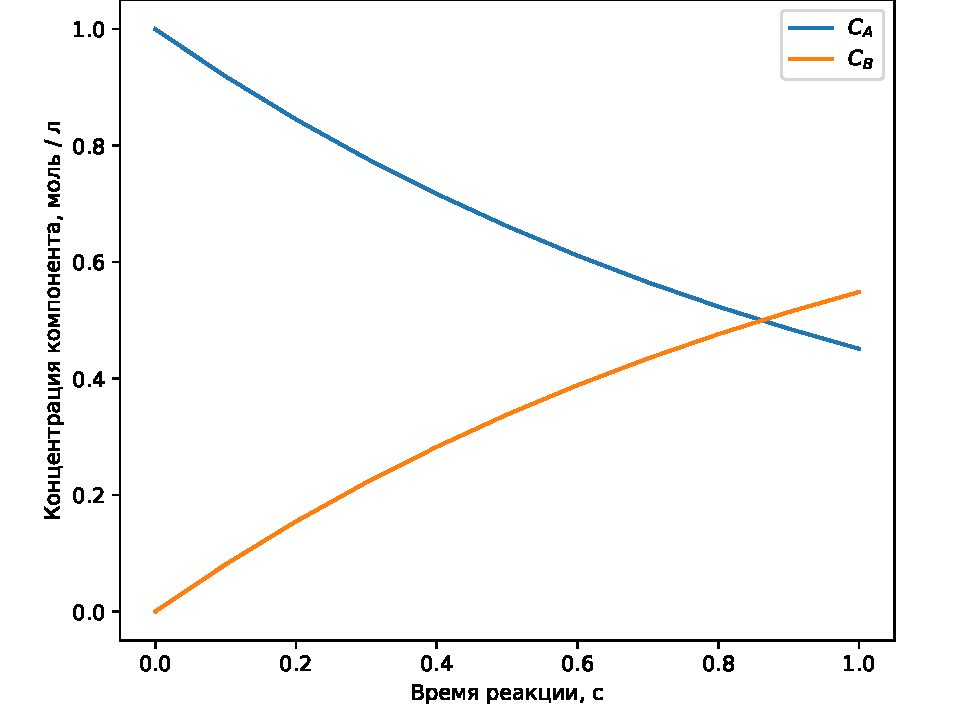
\includegraphics[width=.6\linewidth]{./pics/figure_64}
	\caption{Изменение концентрации реагирующих веществ во времени}
	\label{fig:fig_64}
\end{figure}
\vfill
\end{frame}


\section{Расчет схемы химических реакций}
\begin{frame}[fragile, ]{Расчет схемы химических реакций}
\scriptsize
Рассмотрим следующую схему химических реакций:
\vfill
$$
	A \longleftrightarrow 2B \longleftrightarrow C
$$
\vfill
\noindent с константами скоростей $k_1=0.5$, $k_2=0.8$, $k_3=0.95$ и $k_4=0.1$.
Уравнения, описывающие скорость изменения концентраций компонентов по времени, записываются следующим образом:
\vfill
\begin{minipage}{.49\textwidth}
\begin{enumerate}
\item $A \longrightarrow 2B$ \qquad $r_1 = k_1 \cdot C_A$
\item $2B \longrightarrow A$ \qquad $r_2 = k_2 \cdot C_B ^2$
\item $2B \longrightarrow C$ \qquad $r_3 = k_3 \cdot C_B ^2$
\item $C \longrightarrow 2B$ \qquad $r_4 = k_4 \cdot C_C$
\end{enumerate}
\end{minipage}
\begin{minipage}{.5\textwidth}
\begin{equation*}
	\left\{
	\begin{aligned}
		\dfrac{dC_A}{dt} &= -r_1 + r_2 \\
		\dfrac{dC_B}{dt} &=  2 \cdot \left(r_1 - r_2 - r_3 + r_4\right) \\
		\dfrac{dC_C}{dt} &=  r_3 - r_4 \\
	\end{aligned}
	\right.
\end{equation*}
\end{minipage}
\vfill
$C_{A_0} = 1$, $C_{B_0} = C_{C_0} = 0$ $\mathrm{моль/л}$.
\vfill
\end{frame}


\subsection{Решение методом Эйлера}
\begin{frame}[fragile, ]{Метод Эйлера}
\scriptsize
\begin{minted}{python}
import numpy as np


def func(time: float, c: np.ndarray,
         k: np.ndarray) -> np.ndarray:
    ca, cb, cc = c
    k1, k2, k3, k4 = k
    r1, r2, r3, r4 = [
        k1 * ca,
        k2 * cb ** 2,
        k3 * cb ** 2,
        k4 * cc,
    ]
    dca_dt = -r1 + r2
    dcb_dt = 2 * (r1 - r2 - r3 + r4)
    dcc_dt = r3 - r4

    return dca_dt, dcb_dt, dcc_dt
|\space|
|\space|
\end{minted}
\vfill
\end{frame}


\begin{frame}[fragile, ]{Метод Эйлера}
\scriptsize
\begin{minted}[firstnumber=last]{python}
def eiler(func, x0, xf, y0, h, args=()):
    count = int((xf - x0) / h) + 1
    y = np.zeros((count, y0.shape[0]))
    x, y[0] = x0, y0[:].copy()
    for i in range(1, count):
        right_parts = func(x, y[i-1], *args)
        for j in range(len(y0)):
            y[i][j] = y[i-1][j] + h * right_parts[j]
        x += h
    return y


if __name__ == '__main__':
    k, y0 = np.array([.5, .8, .95, .1]), np.array([1, 0, 0])
    t0, tf, h = 0, 10, .5
    y_eiler = eiler(func, t0, tf, y0, h, args=(k, ))
|\space|
\end{minted}
\vfill
\end{frame}


\subsection{Решение методом Рунге-Кутты}
\begin{frame}[fragile, ]{Метод Рунге-Кутты}
\scriptsize
\begin{minted}{python}
import numpy as np


def func(time: float, c: np.ndarray,
         k: np.ndarray) -> np.ndarray:
    ca, cb, cc = c
    k1, k2, k3, k4 = k
    r1, r2, r3, r4 = [
        k1 * ca,
        k2 * cb ** 2,
        k3 * cb ** 2,
        k4 * cc,
    ]
    dca_dt = -r1 + r2
    dcb_dt = 2 * (r1 - r2 - r3 + r4)
    dcc_dt = r3 - r4

    return dca_dt, dcb_dt, dcc_dt
|\space|
|\space|
\end{minted}
\vfill
\end{frame}


\begin{frame}[fragile, ]{Метод Рунге-Кутты}
\scriptsize
\begin{minted}[firstnumber=last]{python}
def rk(func, x0, xf, y0, h, args=()):
    count = int((xf - x0) / h) + 1
    y = np.zeros((count, y0.shape[0]))
    x, y[0] = x0, y0[:].copy()
    for i in range(1, count):
        k1 = func(x, y[i-1], *args)
        k2 = func(x + h / 2, [y + k * h / 2 for y, k in zip(y[i-1], k1)], *args)
        k3 = func(x + h / 2, [y + k * h / 2 for y, k in zip(y[i-1], k2)], *args)
        k4 = func(x + h, [y + k * h for y, k in zip(y[i-1], k3)], *args)
        for j in range(len(y0)):
            y[i][j] = y[i-1][j] + h / 6 * (k1[j] + 2 * k2[j] + 2 * k3[j] + k4[j])
        x += h
    return y


if __name__ == '__main__':
    k, y0 = np.array([.5, .8, .95, .1]), np.array([1, 0, 0])
    t0, tf, h = 0, 10, .5
    y_rk = rk(func, t0, tf, y0, h, args=(k, ))
|\space|
\end{minted}
\vfill
\end{frame}


\begin{frame}[fragile, ]{Графическая визуализация}
\scriptsize
\begin{figure}
	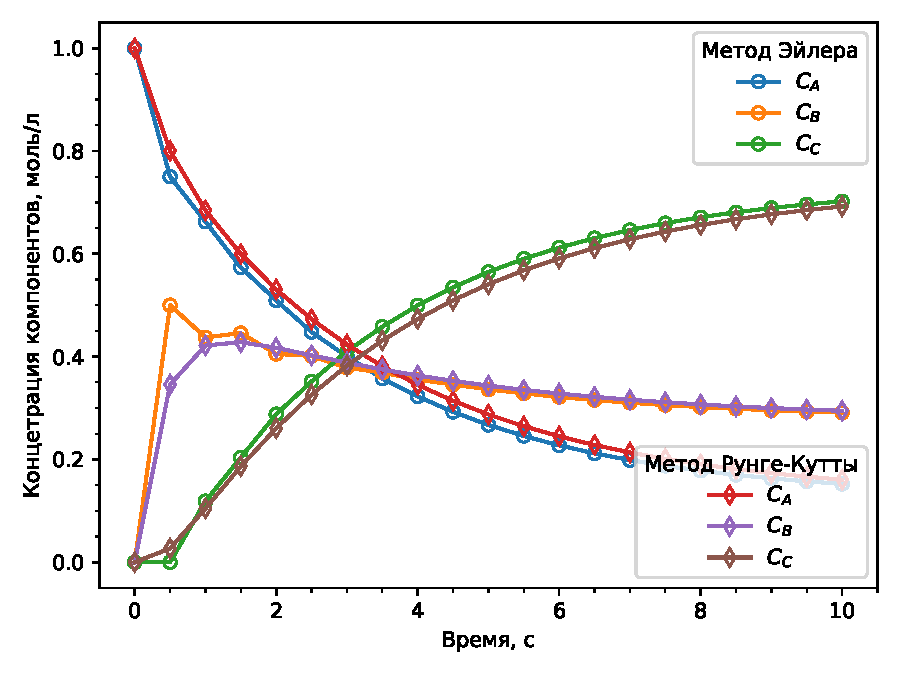
\includegraphics[width=.6\textwidth]{./pics/plot}
	\caption{Изменение концентрации реагирующих веществ по времени}
\end{figure}
\end{frame}


\section{Расчет химической кинетики \\ матричным методом}
\sectionframe

\begin{frame}[fragile, label=c]{Расчет химической кинетики матричным методом}
\scriptsize
Рассмотрим следующую схему химических реакций:
\vfill
$$
	A \longleftrightarrow 2B \longleftrightarrow C
$$
\vfill
\noindent с константами скоростей $k_1=0.5$, $k_2=0.8$, $k_3=0.95$ и $k_4=0.1$.
Уравнения, описывающие скорость изменения концентраций компонентов по времени, записываются следующим образом:
\vfill
\begin{minipage}{.3\textwidth}
\begin{enumerate}
\item $A \longrightarrow 2B$ \quad $r_1 = k_1 \cdot C_A$
\item $2B \longrightarrow A$ \quad $r_2 = k_2 \cdot C_B ^2$
\item $2B \longrightarrow C$ \quad $r_3 = k_3 \cdot C_B ^2$
\item $C \longrightarrow 2B$ \quad $r_4 = k_4 \cdot C_C$
\end{enumerate}
\end{minipage}
\hfill
\begin{minipage}{.3\textwidth}
\begin{equation*}
	\left\{
	\begin{aligned}
		\dfrac{dC_A}{dt} &= -r_1 + r_2 \\
		\dfrac{dC_B}{dt} &=  2 \cdot \left(r_1 - r_2 - r_3 + r_4\right) \\
		\dfrac{dC_C}{dt} &=  r_3 - r_4 \\
	\end{aligned}
	\right.
\end{equation*}
\end{minipage}
\hfill
\begin{minipage}{.3\textwidth}
Стехиометрическая матрица:
\vfill
\begin{table}[h!]
\begin{tabular}{|p{.25\linewidth}|r|r|r|}
\hline
Реакция & $A$ & $B$ & $C$ \\
\hline
$r_1$ & $-1$ &  $2$ &  $0$ \\
\hline
$r_2$ &  $1$ & $-2$ &  $0$ \\
\hline
$r_3$ &  $0$ & $-2$ &  $1$ \\
\hline
$r_4$ &  $0$ &  $2$ & $-1$ \\
\hline
\end{tabular}
\end{table}
\vfill
\end{minipage}
\vfill
$C_{A_0} = 1$, $C_{B_0} = C_{C_0} = 0$ $\mathrm{моль/л}$.
\vfill
\end{frame}


\begin{frame}[fragile, label=c]{Расчет химической кинетики матричным методом}
\scriptsize
\begin{itemize}
\item Зададим матрицу стехиометрических коэффициентов
\begin{minted}[frame=single]{python}
import numpy as np


stoich_matrix = np.array([[-1, 2, 0], [1, -2, 0], [0, -2, 1], [0, 2, -1]])
print(stoich_matrix)
\end{minted}
\vfill
\begin{minted}[frame=none, linenos=false]{pycon}
[[-1  2  0]
 [ 1 -2  0]
 [ 0 -2  1]
 [ 0  2 -1]]
\end{minted}
\vfill
\item Для записи выражений скоростей реакций необходимо из стехиометрической матрицы выбрать элементы с отрицательными коэффициентами. Создадим для этого массив \mintinline{python}|mask|:
\vfill
\begin{minted}[frame=single]{python}
mask = stoich_matrix < 0
print(mask)
\end{minted}
\vfill
\begin{minted}[frame=none, linenos=false]{pycon}
[[ True False False]
 [False  True False]
 [False  True False]
 [False False  True]]
\end{minted}
\end{itemize}
\vfill
\end{frame}


\begin{frame}[fragile, label=c]{Расчет химической кинетики матричным методом}
\scriptsize
\begin{itemize}
\item Зададим значения констант скоростей химических реакций и начальных концентраций компонентов:
\begin{minted}[frame=single]{python}
k = np.array([.5, .8, .95, .1])
c = np.array([1, 0, 0])
\end{minted}
\vfill
\item Вычислим произведение концентраций компонентов в степенях соответствующих стехиометрических коэффициентов для каждой реакции, но только в том случае, если коэффициент $< 0$:
\vfill
\begin{minted}[frame=single]{python}
p = (c ** -(stoich_matrix * mask)).prod(axis=1)
print(p)
\end{minted}
\vfill
\begin{minted}[frame=none, linenos=false]{pycon}
[1.   0.25 0.25 0.2 ]
\end{minted}
\end{itemize}
\vfill
\end{frame}

\begin{frame}[fragile, label=c]{Расчет химической кинетики матричным методом}
\scriptsize
\begin{itemize}
\item Вычислим скорости реакций:
\begin{minted}[frame=single]{python}
reaction_rates = p * k
print(reaction_rates)
\end{minted}
\vfill
\begin{minted}[frame=none, linenos=false]{pycon}
[0.2   0.025 0.025 0.02 ]
\end{minted}
\vfill
\item Правые части дифференциальных уравнений:
\vfill
\begin{minted}[frame=single]{python}
right_parts = (
    (stoich_matrix.T * reaction_rates).sum(axis=1)
)
print(right_parts)
\end{minted}
\vfill
\begin{minted}[frame=none, linenos=false]{pycon}
[-0.175  0.34   0.005]
\end{minted}
\end{itemize}
\vfill
\end{frame}


\begin{frame}[fragile, label=c]{Расчет химической кинетики матричным методом}
\scriptsize
\begin{itemize}
\item Запишем все вышеперечисленное в виде отдельной функции:
\vfill
\begin{minted}{python}
def kinetic_by_matrix(
    time: float,
    c: np.ndarray,
    stoich_matrix: np.ndarray,
    k: np.ndarray
) -> np.ndarray:

    mask = stoich_matrix < 0
    p = (c ** -(stoich_matrix * mask)).prod(axis=1)
    reaction_rates = p * k

    right_parts = (
        (stoich_matrix.T * reaction_rates).sum(axis=1)
    )

    return right_parts
|\space|
\end{minted}
\end{itemize}
\vfill
\end{frame}


\begin{frame}[fragile, label=c]{Расчет химической кинетики матричным методом}
\scriptsize
\begin{itemize}
\item Решим данную систему с использованием функции \mintinline{python}|scipy.integrete.solve_ivp()|:
\vfill
\begin{minted}{python}
from scipy.integrate import solve_ivp


if __name__ == '__main__':
    t = np.linspace(0, 10, 20)  # массив времени
    solution = solve_ivp(
        fun=kinetic_by_matrix,
        t_span=(0, t[-1]),
        y0=c,
        dense_output=True,
        args=(stoich_matrix, k)
    )

    ca, cb, cc = solution.sol(t)
    for a, b, c in zip(ca, cb, cc):
        print(f'{a:>8.4f} {b:>8.4f} {c:>8.4f}')
|\space|
\end{minted}
\end{itemize}
\vfill
\end{frame}


\begin{frame}[fragile, label=c]{Расчет химической кинетики матричным методом}
\scriptsize
Результаты расчета:
\vfill
\begin{minipage}{.35\textwidth}
\begin{minted}[frame=none, linenos=false]{pycon}
  1.0000   0.0000   0.0000
  0.7907   0.3629   0.0278
  0.6716   0.4371   0.1099
  0.5868   0.4322   0.1972
  0.5175   0.4157   0.2746
  0.4591   0.3991   0.3414
  0.4095   0.3841   0.3985
  0.3673   0.3707   0.4473
  0.3315   0.3588   0.4891
  0.3010   0.3482   0.5249
  0.2750   0.3393   0.5554
  0.2529   0.3307   0.5817
  0.2340   0.3241   0.6040
  0.2180   0.3175   0.6232
  0.2042   0.3125   0.6395
  0.1926   0.3077   0.6536
  0.1826   0.3037   0.6656
  0.1740   0.3003   0.6758
  0.1668   0.2969   0.6847
  0.1606   0.2945   0.6922
\end{minted}
\end{minipage}
\begin{minipage}{.64\textwidth}
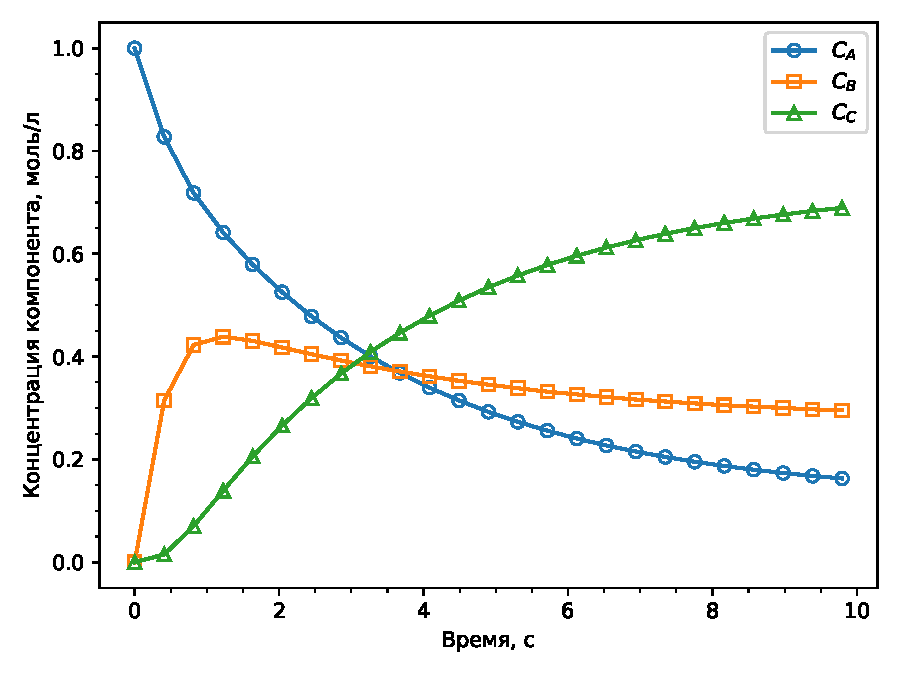
\includegraphics[width=\linewidth]{./pics/fig}
\end{minipage}
\vfill
\end{frame}


\section{Решение обратной кинетической задачи}
\sectionframe

\begin{frame}[fragile, label=c]{Постановка задачи}
\scriptsize
Пусть дана схема реакций:
\vfill
$$
	A \longleftrightarrow 2B \longleftrightarrow C
$$
\vfill
Время протекания процесса $10$~$\mathrm{c}$, концентрации компонентов в момент времени $t = 10$:
\vfill
$$
	C_A = 0.1606 \ \left[\mathrm{моль/л}\right]; \qquad C_B = 0.2945 \ \left[\mathrm{моль/л}\right]; \qquad C_C = 0.6922 \ \left[\mathrm{моль/л}\right].
$$
\vfill
Необходимо найти значения констант скоростей $k_1, \ k_2, \ k_3, \ k_4$, при которых достигаются данные значения концентраций компонентов в заданный момент времени.
\vfill
\end{frame}

\subsection{Метод Нелдера-Мида}
\begin{frame}[fragile, label=c]{Метод Нелдера-Мида}
\scriptsize
Методе Нелдера-Мида доступен как опциональный параметр функции \mintinline{python}|scipy.optimize.minimize()|.

Для применения данной функции потребуется предварительно описать целевую функцию:
\vfill
$$
	error = \sum \limits _{i=1} ^{n} \left(c_i - c_{i, \mathrm{расч.}}\right)^2
$$
\vfill
\end{frame}


\begin{frame}[fragile, label=c]{Метод Нелдера-Мида}
\scriptsize
\begin{minted}{python}
from scipy.optimize import minimize


def obj_func(
    k: np.ndarray, c: np.ndarray,
    kinetic_scheme: callable,
    time: float,
    c0: np.ndarray,
    stoich_matrix: np.ndarray,
) -> float:
    solution = solve_ivp(
        fun=kinetic_by_matrix,
        t_span=(0, time[-1]),
        y0=c0,
        dense_output=True,
        args=(stoich_matrix, k)
    )
    c_calc = solution.sol(time[-1])
    return ((c - c_calc) ** 2).sum()
|\space|
|\space|
\end{minted}
\vfill
\end{frame}


\begin{frame}[fragile, label=c]{Метод Нелдера-Мида}
\scriptsize
\begin{minted}[firstnumber=last]{python}
if __name__ == '__main__':
    c = np.array([.1606, .2945, .6922])
    c0 = np.array([1, 0, 0])
    time = np.linspace(0, 10, 50)
    stoich_matrix = np.array([[-1, 2, 0], [1, -2, 0], [0, -2, 1], [0, 2, -1]])

    initial_k = (.5, .5, .5, .5)
    k = minimize(
        obj_func,
        x0=initial_k,
        args=(
            c,
            kinetic_by_matrix,
            time,
            c0,
            stoich_matrix
        ),
        method='Nelder-Mead'
    )
    print(k)
|\space|
\end{minted}
\vfill
\end{frame}


\begin{frame}[fragile, label=c]{Метод Нелдера-Мида}
\scriptsize
\begin{minted}[frame=none, linenos=false]{pycon}
 final_simplex: (array([[0.40298608, 0.56866624, 0.80859594, 0.07419382],
       [0.40291713, 0.56867713, 0.80862377, 0.07417934],
       [0.40290911, 0.56866281, 0.80862946, 0.07418973],
       [0.40300475, 0.56866888, 0.80856544, 0.07421872],
       [0.40295754, 0.56867751, 0.80859871, 0.07417644]]),
       array([1.61244305e-09, 1.63992065e-09, 1.65274699e-09, 2.05524296e-09,
              2.06513227e-09]))
           fun: 1.612443051432878e-09
       message: 'Optimization terminated successfully.'
          nfev: 142
           nit: 77
        status: 0
       success: True
             x: array([0.40298608, 0.56866624, 0.80859594, 0.07419382])
\end{minted}
\vfill
Действительные значения констант: $k_1=0.5$, $k_2=0.8$, $k_3=0.95$ и $k_4=0.1$.
\vfill
\end{frame}


\subsection{Генетический алгоритм}
\begin{frame}[fragile, label=c]{Генетический алгоритм}
\scriptsize
Для применения генетического алгоритма также понадобится целевая функция и границы изменения искомых констант скоростей химических реакций:
\vfill
\begin{minted}{python}
import genetic_algorithm as ga


bounds = ((.05, 1), (.05, 1), (.05, 1), (.05, 1))  # пределы для искомых значений
k = ga.genetic_algorithm(
    bounds,
    obj_func,
    args=(
        c,
        kinetic_by_matrix,
        time,
        c0,
        stoich_matrix
    ),
    popsize=100,
    selection_size=20,
    generations_count=10
)
print(k[0])
\end{minted}
\vfill
\end{frame}


\begin{frame}[fragile, label=c]{Генетический алгоритм}
\scriptsize
В результате получим следующие значения констант скоростей:
\vfill
\begin{minted}[frame=none, linenos=false]{pycon}
[0.5221326229161222, 0.7950758008292743, 0.8293744138383334, 0.08219397763058496]
\end{minted}
\vfill
Данные значения можно улучшить, еще раз применив генетический алгоритм или метод Нелдера-Мида с полученным решением в качестве начального приближения:
\vfill
\begin{minted}{python}
initial_k = [
    0.5221326229161222, 0.7950758008292743,
    0.8293744138383334, 0.08219397763058496
]
k = minimize(
    obj_func,
    x0=initial_k,
    args=(
        c,
        kinetic_by_matrix,
        time,
        c0,
        stoich_matrix
    ),
    method='Nelder-Mead'
)
print(k)
\end{minted}
\vfill
\end{frame}


\begin{frame}[fragile, label=c]{Генетический алгоритм}
\scriptsize
Повторное применение метода Нелдера-Мида после генетического алгоритма, дает следующее решение:
\vfill
\begin{minted}[frame=none, linenos=false]{pycon}
 final_simplex: (array([[0.51709669, 0.81808365, 0.83553017, 0.08311357],
       [0.51713805, 0.81815404, 0.83548288, 0.08311136],
       [0.51711343, 0.81803742, 0.83551075, 0.08311706],
       [0.51706307, 0.81800744, 0.83555168, 0.08312275],
       [0.51711475, 0.81804012, 0.835535  , 0.08311974]]),
       array([1.14057758e-09, 1.14544246e-09, 1.17218242e-09, 1.21210320e-09,
              1.21655242e-09]))
           fun: 1.1405775778538453e-09
       message: 'Optimization terminated successfully.'
          nfev: 85
           nit: 43
        status: 0
       success: True
             x: array([0.51709669, 0.81808365, 0.83553017, 0.08311357])
\end{minted}
\vfill
Действительные значения констант: $k_1=0.5$, $k_2=0.8$, $k_3=0.95$ и $k_4=0.1$.
\vfill
\end{frame}


\contactsframe[\Large \textbf{Благодарю за внимание!}]{

    \bigskip
    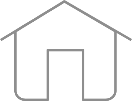
\includegraphics[width=.05\textwidth]{pics/home} \quad Учебный корпус №2, ауд. 136 \\
    
\includegraphics[width=.05\textwidth]{pics/mail} \quad chuva@tpu.ru \\
    
\includegraphics[width=.03\textwidth]{pics/tel} \quad +7-962-782-66-15
}

\end{document}

